\subsection{Activity Type Graph}
\label{sec:ATG}
When a Recruiter makes a request to one of the Archivists, the Archivist has to somehow choose the relevant Educators. Moreover, when an Educator discloses the data, it has to provide as minimal set of entries as possible. This set has to be verifiable, which means that the Educator provides the proof of the data validity along with the data being disclosed.

In order to achieve these goals, we divide the data that the Educators store into atomic Activity Types. Each Educator maintains a journal of transactions per each Activity Type that the Educator offers.

All the Activity Types are grouped into courses that are further grouped into larger entities such as subjects and areas of knowledge. This grouping can be stored as the Activity Type Graph $G_A$ with the following properties:
\begin{enumerate}[label=\arabic*${}^\circ$]
\item $G_A$ is a directed graph:
  \begin{equation}
  G_A:\ \langle V: \{\mathrm{Vert}\},\ e_{out}: \mathrm{Vert} \rightarrow \{\mathrm{Vert}\}\ |\ \mathrm{rest} \rangle
  \end{equation}

\item Each vertex of $G_A$ is associated with depth:
  \begin{equation}
  G_A:\ \langle d: \mathrm{Vert} \rightarrow \mathrm{Int}\ |\ \mathrm{rest}  \rangle
  \end{equation}

\item Law of pointing down:
  \begin{equation}
  G_A:\ \langle v \in e_{out}(u) \implies d(v) > d(u) \rangle
  \end{equation}

\item $G_A$ has special \textit{et cetera} vertices $u$:
  \begin{equation}
  \forall\ v \in V\ \exists u\ (u \in e_{out}(v) \land e_{out}(u) = \emptyset)
  \end{equation}
\end{enumerate}

The example of the Activity Type Graph (ATG) is shown in Figure~\ref{fig:atg}. The vertex $v$ of the graph is a \textit{leaf} if $e_{out}(v) = \emptyset$. Otherwise we call it an \textit{internal vertex}. Every internal vertex of the graph has a special \textit{etc.} child (some of these are ommitted in the figure).

\begin{figure}[ht]
\centering
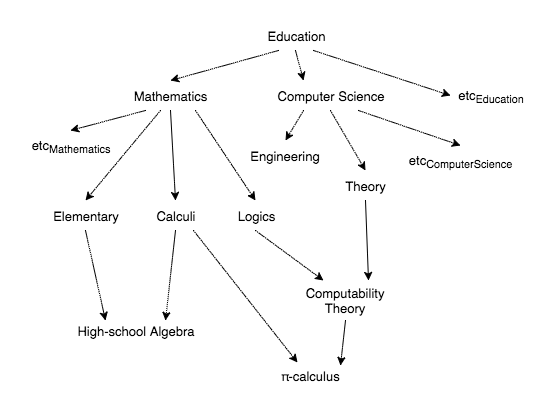
\includegraphics[width=0.8\textwidth]{atg}
\caption{An example of the Activity Type Graph. Some of the vertices are not shown}
\label{fig:atg}
\end{figure}

The need for \textit{etc.} vertices arises from the fact that not all of the Educators teach courses exactly in leaves — some of them offer general courses that provide just the necessary background. For example, some of the universities teach the basic \textquote{Computer science} course, that contains the basics of the discipline. In this case, when the particular category is hard to define, the university would use the $\textrm{etc}_{\textrm{ComputerScience}}$ vertex.

On the protocol level, the Educators can announce that they teach a particular course, but can not modify the Activity Type Graph structure. The structure of the graph is maintained by the core developers and updated upon request from the Educators.

For every pair of vertices $(v, u)$, $weight(v, u)$ defines how the score of a course from the field of study $u$ affects the summary grade for the field of study $v$. Let's define $weight(v, u) = \frac{1}{d(u) - d(v) + 1}$ if $u$ reachable from $v$, and $weight(v, u) = 0$ otherwise. The motivation of the aforementioned weights is that less specific subject implies the wider knowledge. After that we can define $avgGrades_{subjectId}$ as a weighted average with weights described above.
